\documentclass[11pt]{article}

\usepackage[margin=1in]{geometry}
\usepackage[T1]{fontenc}
\usepackage{lmodern}
\usepackage{microtype}
\usepackage{amsmath,amssymb,amsthm,mathtools}
\usepackage[dvipsnames]{xcolor}
\usepackage[most]{tcolorbox}
\usepackage{tikz}
\usetikzlibrary{decorations.markings}
\usepackage{enumitem}
\usepackage{tocloft}
\usepackage[hidelinks]{hyperref}

\definecolor{courseblue}{HTML}{1F4E79}
\definecolor{lightblue}{HTML}{EAF2F8}
\definecolor{lightgreen}{HTML}{EAF7EA}
\definecolor{lightpink}{HTML}{FCE8EF}
\definecolor{lightyellow}{HTML}{FFF8D6}
\definecolor{warningyellow}{HTML}{D6A000}
\definecolor{exercisebg}{HTML}{D6E6F5}
\definecolor{exerciseframe}{HTML}{1F4E79}
\definecolor{examplebg}{HTML}{F4FAFE}
\definecolor{exampleframe}{HTML}{85C1E9}
\definecolor{darkgray}{HTML}{333333}
\definecolor{lightorange}{HTML}{FDEBD8}
\definecolor{orangeframe}{HTML}{E08A3C}

\setlength{\parindent}{0pt}
\setlength{\parskip}{0.65em}
\setlist[itemize]{topsep=0.25em,itemsep=0.15em}
\renewcommand{\cftsecleader}{\cftdotfill{\cftdotsep}}
\renewcommand{\cftsubsecleader}{\cftdotfill{\cftdotsep}}

\theoremstyle{plain}
\newtheorem{theorem}{Theorem}[section]
\newtheorem{proposition}[theorem]{Proposition}
\newtheorem{lemma}[theorem]{Lemma}
\newtheorem{corollary}[theorem]{Corollary}
\theoremstyle{definition}
\newtheorem{definition}[theorem]{Definition}
\newtheorem{example}[theorem]{Example}
\newtheorem{exercise}[theorem]{Exercise}
\theoremstyle{remark}
\newtheorem*{remark}{Remark}
\newtheorem*{fact}{Fact}
\newtheorem*{warning}{Warning}

\tcolorboxenvironment{definition}{
  enhanced,
  unbreakable,
  colback=lightgreen,
  colframe=ForestGreen,
  boxrule=0.7pt,
  arc=2pt,
  left=6pt,
  right=6pt,
  top=5pt,
  bottom=5pt
}

\tcolorboxenvironment{warning}{
  enhanced,
  colback=lightyellow,
  colframe=warningyellow,
  boxrule=0.7pt,
  arc=2pt,
  left=6pt,
  right=6pt,
  top=5pt,
  bottom=5pt
}

\tcolorboxenvironment{exercise}{
  enhanced,
  colback=exercisebg,
  colframe=exerciseframe,
  boxrule=1pt,
  arc=2pt,
  left=6pt,
  right=6pt,
  top=5pt,
  bottom=5pt
}

\tcolorboxenvironment{example}{
  enhanced,
  colback=examplebg,
  colframe=exampleframe,
  boxrule=0.7pt,
  arc=2pt,
  left=6pt,
  right=6pt,
  top=5pt,
  bottom=5pt
}

\numberwithin{equation}{section}

\newcommand{\be}{\begin{eqnarray}}
\newcommand{\ee}{\end{eqnarray}}
\newcommand{\C}{\mathbb{C}}
\newcommand{\R}{\mathbb{R}}
\newcommand{\N}{\mathbb{N}}

\DeclareMathOperator{\Hol}{\mathcal{H}\mathrm{ol}}
\DeclareMathOperator{\Real}{Re}
\DeclareMathOperator{\Imag}{Im}
\newcommand{\A}{\mathcal{A}}
\newcommand{\CT}{\C[[T]]}
\newcommand{\CLT}{\C((T))}
\tcbset{breakable}
\begin{document}

\begin{center}
  \colorbox{lightblue}{%
    \begin{minipage}{0.94\textwidth}
      \vspace{0.55em}
      \begin{tabular*}{\textwidth}{@{\extracolsep{\fill}}lr}
        {\color{courseblue}\bfseries\LARGE Lecture 11} &
        {\color{courseblue}\bfseries\LARGE MATH 411}\\[0.35em]
        \textbf{Fall 2026} & \textbf{Date: Sep 28, 2026}\\
        & \textbf{Instructor: Manish Patnaik}
      \end{tabular*}
      \vspace{0.45em}
    \end{minipage}}
\end{center}

\setcounter{tocdepth}{1}
\tableofcontents
\vspace{0.45em}

% Handwritten page 1.
\section{Analytic extensions of real functions}
Recall from Lecture~10 that if two convergent power series agree on an infinite set
accumulating at $0$, they are equal as power series.

Let $f(x)$ be a real-valued function on an interval $(-c,c)\subseteq\R$.

\noindent
\begin{minipage}[c]{0.66\textwidth}
\begin{definition}[Extension]
We call a function $g$, defined on a neighbourhood of $0$ in $\C$, an
\emph{extension} of $f$ if $g(x)=f(x)$ for all real $x\in(-\varepsilon,\varepsilon)$, for some $\varepsilon > 0$.
\end{definition}
\end{minipage}\hfill
\begin{minipage}[c]{0.3\textwidth}
\centering
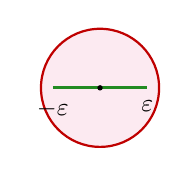
\begin{tikzpicture}[scale=0.75]
  \fill[lightpink,opacity=0.9] (0,0) circle (1);
  \draw[red!75!black,thick] (0,0) circle (1);
  \draw[ForestGreen,very thick] (-0.8,0) -- (0.8,0);
  \node[below,font=\small] at (-0.8,-0.05) {$-\varepsilon$};
  \node[below,font=\small] at (0.8,-0.05) {$\varepsilon$};
  \fill (0,0) circle (1.3pt);
\end{tikzpicture}
\end{minipage}

\begin{corollary}
\label{cor:unique-ext}
There is at most one analytic function around $0$ which restricts to
$f(x)$. More precisely, if $g_1$ and $g_2$ are analytic extensions of $f$,
then $g_1=g_2$ on some disc around $0$.
\end{corollary}

\begin{proof}
Near $0$, write $g_1(z)=\sum a_nz^n$ and $g_2(z)=\sum b_nz^n$ with positive
radii of convergence. These agree at the points $x=1/n$ for all large $n$,
which accumulate at $0$. By the identity principle from Lecture~10,
$\sum a_nT^n=\sum b_nT^n$, so $g_1=g_2$ on a common disc of convergence.
\end{proof}

\begin{warning}
We are not saying that such an extension exists, just that it is unique if
it does exist.
\end{warning}

\begin{example}[The exponential]
\label{ex:exp}
The function $e^x$ defined on $\R$ has at most one analytic extension.
Consider
\be
 \operatorname{Exp}(z)=\sum_{n=0}^{\infty}\frac{z^n}{n!},
\ee
which has infinite radius of convergence. On the real line it restricts to
$e^x$, by the usual power series expansion of $e^x$ from calculus. So
$\operatorname{Exp}(z)$ is \emph{the} analytic extension of $e^x$.

On the other hand, we previously defined, for $z=x+iy$,
\be
 e^z=e^x e^{iy}=e^x(\cos y+i\sin y).
\ee
\emph{Question.} What is the relation between $\operatorname{Exp}(z)$ and
$e^z$?

Note:
\begin{enumerate}[label=(\arabic*)]
  \item $e^ze^w=e^{z+w}$, and likewise
  $\operatorname{Exp}(z)\operatorname{Exp}(w)=\operatorname{Exp}(z+w)$.
  (For the latter, multiply the two absolutely convergent series and use the
  binomial theorem: the coefficient of the degree-$n$ part of the product is
  $\sum_{k}\frac{z^kw^{n-k}}{k!(n-k)!}=\frac{(z+w)^n}{n!}$.)
  \item $\operatorname{Exp}(x)=e^x$ on the real line.
  \item \emph{Check:} $\operatorname{Exp}(iy)=e^{iy}$.
\end{enumerate}

For (3), plug $z=iy$ into the definition and separate even and odd powers
(allowed since the series converges absolutely), using $i^{2n}=(-1)^n$ and
$i^{2n+1}=(-1)^ni$:
\be
 \operatorname{Exp}(iy)
 =\underbrace{\sum_{n=0}^{\infty}(-1)^n\frac{y^{2n}}{(2n)!}}_{\cos y}
 +\,i\underbrace{\sum_{n=0}^{\infty}(-1)^n\frac{y^{2n+1}}{(2n+1)!}}_{\sin y}.
\ee
Therefore $\operatorname{Exp}(iy)=\cos y+i\sin y$. Combining (1)--(3),
\be
 \operatorname{Exp}(x+iy)=\operatorname{Exp}(x)\operatorname{Exp}(iy)
 =e^x(\cos y+i\sin y)=e^{x+iy},
\ee
so $\operatorname{Exp}(z)=e^z$ for all $z\in\C$.
\end{example}
%
%\section{The binomial series}
%\begin{definition}
%For $\alpha\in\C$ and $n$ a non-negative integer, set
%\be
% \binom\alpha n=\frac{\alpha(\alpha-1)\cdots(\alpha-n+1)}{n!},
% \qquad \binom\alpha0=1.
%\ee
%The \emph{binomial series} is
%\be
% B_\alpha(T)=\sum_{n=0}^{\infty}\binom\alpha n T^n\in\CT.
%\ee
%\end{definition}
%
%\begin{proposition}
%\label{prop:binom-analytic}
%If $\alpha$ is a non-negative integer, $B_\alpha(T)$ has infinite radius
%of convergence; otherwise its radius is $1$. In either case it defines
%an analytic function on $D(0,1)$.
%\end{proposition}
%
%\begin{proof}
%\textbf{Case $\alpha=m$ a non-negative integer.} Then eventually
%$\binom\alpha n=0$, since
%\be
% \binom mn=0\qquad\text{if }m<n
%\ee
%(the numerator contains the factor $m-m=0$). So $B_m(T)$ is a polynomial,
%its radius of convergence is $\infty$, and moreover, by the binomial theorem,
%\be
% B_m(T)=(1+T)^m.
%\ee
%
%\textbf{Case $\alpha$ is not a non-negative integer.} Then no coefficient vanishes, and the ratio
%test gives
%\be
% \left|\binom\alpha{n+1}\Big/\binom\alpha n\right|
% =\frac{|\alpha-n|}{n+1}\longrightarrow1
% \qquad(n\to\infty),
%\ee
%so the radius of convergence is $1$.
%In either case $B_\alpha(T)$ converges on $D(0,1)$, so by Lecture~9
%the function $B_\alpha(z)$ is analytic there.
%\end{proof}
%
%\emph{What is $B_\alpha(z)$?} Take $\alpha=\frac1m$ with $m\in\N$, $m\geq1$.
%
%\begin{theorem}
%\label{thm:mth-root}
%$B_{1/m}(z)$ is the analytic $m$-th root of $1+z$ on $D(0,1)$ that equals
%$1$ at $z=0$. In particular,
%\be
% B_{1/m}(z)^m=1+z\qquad\text{for all }z\in D(0,1).
%\ee
%\end{theorem}
%
%\emph{Idea.} Both $B_{1/m}(z)^m$ and $1+z$ are analytic extensions of the
%same function on the reals. That is, we want to show
%\be
% (1+x)^{1/m}=B_{1/m}(x)\qquad\text{for }x\in(-1,1).
% \label{eq:real-root}
%\ee
%Put $f(x)=(1+x)^{1/m}$. Calculus gives
%\be
% f'(x)=\tfrac1m(1+x)^{\frac1m-1},\qquad
% f''(x)=\tfrac1m\bigl(\tfrac1m-1\bigr)(1+x)^{\frac1m-2},\qquad\dots,
%\ee
%and in general $f^{(n)}(0)=n!\binom{1/m}{n}$. To verify that its Taylor
%series equals $f$, put $b_n=\binom{1/m}{n}$. The recurrence
%$(n+1)b_{n+1}=(\frac1m-n)b_n$ and termwise differentiation give
%\be
% (1+x)B_{1/m}'(x)=\tfrac1m B_{1/m}(x)\qquad(|x|<1).
%\ee
%Since $f$ satisfies the same equation and $f(x)>0$ on $(-1,1)$,
%the quotient $B_{1/m}(x)/f(x)$ has derivative zero. It equals $1$ at
%$x=0$, proving \eqref{eq:real-root} and hence
%$B_{1/m}(x)^m=1+x$ for real $x\in(-1,1)$.
%
%To pass from real $x$ to complex $z$ we want to apply the identity principle
%to $B_{1/m}(T)^m$ and $1+T$. For that we need to know that the formal
%product of convergent power series is again convergent, and that it computes
%the product of the functions. This is the content of the next section.

% Handwritten page 5.
\section{Path integrals and Cauchy's theorems}
\subsection*{Integrating complex-valued functions of a real variable}
Let $F\colon[a,b]\to\C$, and write $F(t)=u(t)+iv(t)$ with $u$, $v$
real-valued. We define
\be
 \int_a^bF(t)\,dt=\int_a^bu(t)\,dt+i\int_a^bv(t)\,dt,
\ee
which takes $\C$-values. All the familiar rules carry over by working with
real and imaginary parts.

\begin{exercise}
Check that if $F$ and $G$ have continuously differentiable real and
imaginary parts, then integration by parts holds:
\be
 \int_a^bF(t)\,G'(t)\,dt=\Bigl[F(t)\,G(t)\Bigr]_a^b-\int_a^bG(t)\,F'(t)\,dt.
\ee
Also, the ``Fundamental Theorem of Calculus'' (FTC) holds: if $F$ is continuous, then
$s\mapsto\int_a^sF(t)\,dt$ has derivative $F(s)$ for $s\in(a,b)$ (with
one-sided derivatives at the endpoints).
\end{exercise}

\begin{proposition}[Basic estimate]
\label{prop:basic-est}
For continuous $F\colon[a,b]\to\C$,
\be
 \left|\int_a^bF(t)\,dt\right|\leq\int_a^b|F(t)|\,dt.
\ee
\end{proposition}

\begin{proof}
Let $I=\int_a^bF(t)\,dt$ and write $I=|I|e^{i\theta}$. Then
\be
 |I|=e^{-i\theta}I=\int_a^b e^{-i\theta}F(t)\,dt
 =\int_a^b\Real\bigl(e^{-i\theta}F(t)\bigr)\,dt
 \leq\int_a^b|F(t)|\,dt,
\ee
where the third equality holds because $|I|$ is real, so the imaginary part
of the integral vanishes.
\end{proof}

\subsection*{Integrating along a path}
More interesting: let $U\subseteq\C$ be open and $f$ a function on $U$.

\begin{definition}[Piecewise continuously differentiable path]
A curve $\gamma\colon[a,b]\to U$ is \emph{piecewise continuously differentiable}
if it is continuous on $[a,b]$ and there is a finite partition
$a=t_0<t_1<\cdots<t_m=b$ such that $\gamma$ is continuously differentiable
on each $[t_{j-1},t_j]$, with one-sided derivatives at the endpoints.
Unless said otherwise, a \emph{path} means such a curve. Its derivative
need not exist at the joining points $t_1,\ldots,t_{m-1}$.
\end{definition}

\begin{center}
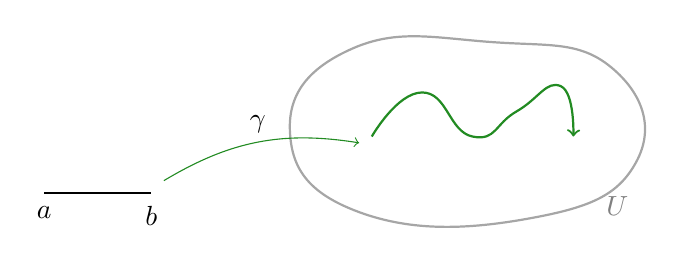
\begin{tikzpicture}[scale=0.8]
  \draw[thick,gray!70] plot[smooth cycle,tension=0.8]
    coordinates {(-2.6,0.2) (-1.6,1.5) (0.6,1.6) (2.5,1.2) (2.9,-0.3) (1.2,-1.2) (-1.5,-1.1)};
  \draw[ForestGreen,thick,->] plot[smooth,tension=0.9]
    coordinates {(-1.3,0.1) (-0.5,0.8) (0.3,0.1) (1.0,0.5) (1.7,0.9) (1.9,0.1)};
  \node[gray] at (2.6,-1.0) {$U$};
  \draw[thick] (-6.5,-0.8) -- (-4.8,-0.8);
  \node[below] at (-6.5,-0.85) {$a$};
  \node[below] at (-4.8,-0.85) {$b$};
  \draw[->,ForestGreen] (-4.6,-0.6) to[bend left=20] node[above,black]{$\gamma$} (-1.5,0.0);
\end{tikzpicture}
\end{center}

% Handwritten page 6.
\begin{definition}[Path integral]
\label{def:path-int}
For $f$ continuous on $U$ and $\gamma\colon[a,b]\to U$ a path, write
$\gamma(t)=u(t)+iv(t)$, so $\gamma'(t)=u'(t)+iv'(t)$ on each $C^1$ piece. Then
\be
 \int_\gamma f=\int_\gamma f\,dz:=\int_a^bf\bigl(\gamma(t)\bigr)\,\gamma'(t)\,dt.
\ee
\end{definition}

\begin{example}
\label{ex:circle}
Let $\gamma(\theta)=\cos\theta+i\sin\theta=e^{i\theta}$ for
$\theta\in[0,2\pi]$, and $f(z)=\frac1z$. Then $\gamma'(\theta)=ie^{i\theta}$,
so
\be
 \int_\gamma f=\int_0^{2\pi}f\bigl(\gamma(\theta)\bigr)\,\gamma'(\theta)\,d\theta
 =\int_0^{2\pi}\frac1{e^{i\theta}}\,ie^{i\theta}\,d\theta
 =2\pi i.
\ee
\end{example}

\begin{remark}\leavevmode
\begin{enumerate}[label=(\arabic*)]
  \item \emph{What happens if we change orientation?} For
  $\gamma(\theta)=e^{-i\theta}$, $\theta\in[0,2\pi]$, the same computation
  gives
  \be
   \int_\gamma\frac{dz}{z}=\int_0^{2\pi}\frac{-ie^{-i\theta}}{e^{-i\theta}}\,d\theta=-2\pi i.
  \ee
  So orientation matters.
  \item \begin{minipage}[t]{\linewidth}
  \emph{What if we replace $\gamma(\theta)$ with
  $\gamma_R(\theta)=Re^{i\theta}$?} Then
  \be
   \int_{\gamma_R}\frac{dz}z=\int_0^{2\pi}\frac1{Re^{i\theta}}\,Rie^{i\theta}\,d\theta=2\pi i,
  \ee
  independently of $R$. We will see later that the answer is the same for
  any closed path winding once counterclockwise around $0$.
  \begin{center}
  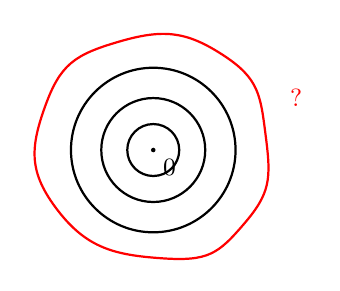
\begin{tikzpicture}[scale=0.55]
    \foreach \r in {0.6,1.2,1.9} \draw[thick] (0,0) circle (\r);
    \fill (0,0) circle (1.5pt) node[below right,font=\small]{$0$};
    \draw[red,thick] plot[smooth cycle,tension=0.9]
      coordinates {(2.6,0.3) (1.6,2.2) (-0.8,2.5) (-2.5,1.0) (-2.2,-1.4) (0.2,-2.5) (2.1,-1.7)};
    \node[red,font=\small] at (3.3,1.2) {?};
  \end{tikzpicture}
  \end{center}
  \end{minipage}
\end{enumerate}
\end{remark}
%
%\begin{example}
%\label{ex:rect}
%Let $\gamma=\gamma_1\cup\gamma_2\cup\gamma_3\cup\gamma_4$ be the boundary of a
%rectangle containing $0$, traversed counterclockwise, so that
%\be
% \int_\gamma f=\sum_{i=1}^{4}\int_{\gamma_i}f.
%\ee
%
%\noindent
%\begin{minipage}[c]{0.4\textwidth}
%\centering
%\begin{tikzpicture}[scale=0.8,decoration={markings,mark=at position 0.55 with {\arrow{>}}}]
%  \draw[thick,postaction={decorate}] (-1.5,-1) -- (1.5,-1) node[midway,below]{$\gamma_1$};
%  \draw[thick,postaction={decorate}] (1.5,-1) -- (1.5,1) node[midway,right]{$\gamma_2$};
%  \draw[thick,postaction={decorate}] (1.5,1) -- (-1.5,1) node[midway,above]{$\gamma_3$};
%  \draw[thick,postaction={decorate}] (-1.5,1) -- (-1.5,-1) node[midway,left]{$\gamma_4$};
%  \fill (0,0) circle (1.4pt) node[right]{$0$};
%\end{tikzpicture}
%\end{minipage}\hfill
%\begin{minipage}[c]{0.56\textwidth}
%Pick $f=1$. Then $\int_\gamma 1=0$. Similarly $\int_\gamma z\,dz=0$.
%\end{minipage}
%\end{example}

\subsection*{The unit square}
\begin{example}
\label{ex:unit-square}
Let $\gamma=\gamma_1\cup\gamma_2\cup\gamma_3\cup\gamma_4$ be the boundary of
the unit square with vertices $0,1,1+i,i$, traversed counterclockwise. What
is $\int_\gamma1$? Parametrize each side by $0\leq t\leq1$:

\noindent
\begin{minipage}[c]{0.36\textwidth}
\centering
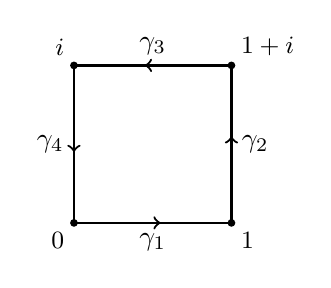
\begin{tikzpicture}[scale=2.0,decoration={markings,mark=at position 0.55 with {\arrow{>}}}]
  \draw[thick,postaction={decorate}] (0,0) -- (1,0) node[midway,below]{$\gamma_1$};
  \draw[thick,postaction={decorate}] (1,0) -- (1,1) node[midway,right]{$\gamma_2$};
  \draw[thick,postaction={decorate}] (1,1) -- (0,1) node[midway,above]{$\gamma_3$};
  \draw[thick,postaction={decorate}] (0,1) -- (0,0) node[midway,left]{$\gamma_4$};
  \foreach \p/\l/\a in {{(0,0)}/0/below left,{(1,0)}/1/below right,{(1,1)}/1+i/above right,{(0,1)}/i/above left}
    \fill \p circle (0.7pt) node[\a,font=\small]{$\l$};
\end{tikzpicture}
\end{minipage}\hfill
\begin{minipage}[c]{0.6\textwidth}
\begin{center}
\renewcommand{\arraystretch}{1.25}
\begin{tabular}{lll}
 & $\gamma_j(t)$ & $\gamma_j'(t)$\\\hline
 $\gamma_1$ & $t$ & $1$\\
 $\gamma_2$ & $1+it$ & $i$\\
 $\gamma_3$ & $(1-t)+i$ & $-1$\\
 $\gamma_4$ & $(1-t)i$ & $-i$
\end{tabular}
\end{center}
\end{minipage}

Then
\be
 \int_\gamma1=\underbrace{\int_0^11\,dt}_{\gamma_1}+\underbrace{\int_0^1i\,dt}_{\gamma_2}
 +\underbrace{\int_0^1(-1)\,dt}_{\gamma_3}+\underbrace{\int_0^1(-i)\,dt}_{\gamma_4}=0.
\ee
\end{example}

\begin{exercise}
With $\gamma$ as in Example~\ref{ex:unit-square}, show that
$\int_\gamma z\,dz=0$.
\end{exercise}

\subsection*{Further properties of path integrals}
\begin{proposition}[Independence of parametrization]
\label{prop:reparam}
Let $\psi\colon[c,d]\to U$ be a path and let $g\colon[a,b]\to[c,d]$ be
continuously differentiable with $g(a)=c$ and $g(b)=d$. Set
$\gamma=\psi\circ g\colon[a,b]\to U$, i.e.\ $\gamma(t)=\psi\bigl(g(t)\bigr)$. Then
\be
 \int_\gamma f=\int_\psi f.
\ee
\end{proposition}

\begin{center}
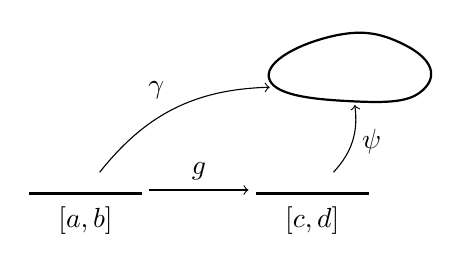
\begin{tikzpicture}[scale=0.9]
  \draw[thick] (0,0) -- (1.6,0);
  \node[below] at (0.8,-0.05) {$[a,b]$};
  \draw[thick] (3.2,0) -- (4.8,0);
  \node[below] at (4.0,-0.05) {$[c,d]$};
  \draw[->] (1.7,0.05) -- node[above]{$g$} (3.1,0.05);
  \draw[thick] plot[smooth cycle,tension=0.9]
    coordinates {(3.4,1.6) (4.2,2.2) (5.3,2.1) (5.6,1.5) (4.6,1.3)};
  \draw[->] (1.0,0.3) to[bend left=25] node[above left]{$\gamma$} (3.4,1.5);
  \draw[->] (4.3,0.3) to[bend right=25] node[right]{$\psi$} (4.6,1.25);
\end{tikzpicture}
\end{center}

\begin{proof}
By the chain rule $\gamma'(t)=\psi'\bigl(g(t)\bigr)g'(t)$, so substituting
$s=g(t)$,
\be
 \int_\gamma f=\int_a^bf\bigl(\psi(g(t))\bigr)\,\psi'\bigl(g(t)\bigr)\,g'(t)\,dt
 =\int_c^df\bigl(\psi(s)\bigr)\,\psi'(s)\,ds=\int_\psi f.
\ee
(Apply the real change-of-variables formula to real and imaginary parts.)
\end{proof}

\begin{proposition}
\label{prop:ML}
For a path $\gamma\colon[a,b]\to\C$, let
\be
 L(\gamma)=\text{arclength of }\gamma=\int_a^b|\gamma'(t)|\,dt.
\ee
Then
\be
 \left|\int_\gamma f\right|\leq\Bigl(\sup_{z\in\gamma([a,b])}|f(z)|\Bigr)\cdot L(\gamma).
\ee
\end{proposition}

\begin{proof}
Why? Since $\int_\gamma f=\int_a^bf\bigl(\gamma(t)\bigr)\,\gamma'(t)\,dt$, the
basic estimate above gives
\be
 \left|\int_\gamma f\right|\leq\int_a^b\bigl|f\bigl(\gamma(t)\bigr)\bigr|\,|\gamma'(t)|\,dt
 \leq\sup_{z\in\gamma([a,b])}|f(z)|\int_a^b|\gamma'(t)|\,dt.
\ee
\end{proof}

We will also use the following simple observation.

\begin{lemma}
\label{lem:poly-closed}
If $Q$ is a polynomial and $\gamma\colon[a,b]\to\C$ is a closed path
($\gamma(a)=\gamma(b)$), then $\int_\gamma Q(z)\,dz=0$. In particular
$\int_\gamma c\,dz=0$ and $\int_\gamma(z-z_0)\,dz=0$ for any constants
$c,z_0\in\C$.
\end{lemma}

\begin{proof}
By linearity it suffices to take $Q(z)=z^n$ for $n\geq0$. Choose a partition
$a=t_0<\cdots<t_m=b$ on whose pieces $\gamma$ is $C^1$. On each piece the
chain rule gives
$\frac{d}{dt}\bigl(\gamma(t)^{n+1}/(n+1)\bigr)=\gamma(t)^n\gamma'(t)$.
Applying the Fundamental Theorem of Calculus on each piece and summing, the
intermediate endpoint terms cancel:
\be
 \int_\gamma z^n\,dz
 =\sum_{j=1}^m\int_{t_{j-1}}^{t_j}\gamma(t)^n\gamma'(t)\,dt
 =\frac{\gamma(b)^{n+1}-\gamma(a)^{n+1}}{n+1}=0.
\ee
The last statement follows by taking $Q(z)=c$ and $Q(z)=z-z_0$.
\end{proof}

We will prove next time:

\begin{theorem}[Cauchy--Goursat]
Let $f$ be holomorphic on an open set $U$, and let $R$ be a rectangle with
$R\subseteq U$. Then
\be
 \int_{\partial R}f=0.
\ee
\end{theorem}

\end{document}
